	\begin{tikzpicture}
	[every label/.append style={text=Orange, font=\scriptsize,opacity=0.7},
	ttt/.style={font=\scriptsize}
	]
	
	% The last trick is to cheat and use transparency
	\begin{scope}
	%	\fill[red] \firstcircle;
	%	\fill[green] \secondcircle;
	%	\fill[blue] \thirdcircle;
	\draw \firstcircle node[above left , text=brown, xshift=0.5cm] 
	{\textbf{Conception 3D web}};
\draw node[xshift=-1cm,yshift=-0.5cm,align=center] { 

\includegraphics[width=1.5cm]{cube.png}};

\node at (2,-1){? };
%	\draw \secondcircle node [above right, align=center] {
%	 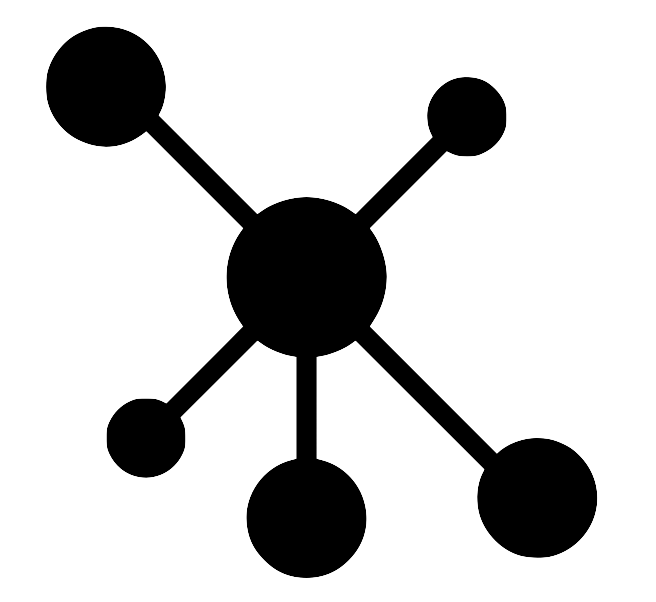
\includegraphics[width=1cm]{img/network.png}
%};
%	\draw \thirdcircle node [below, align=center] 
%{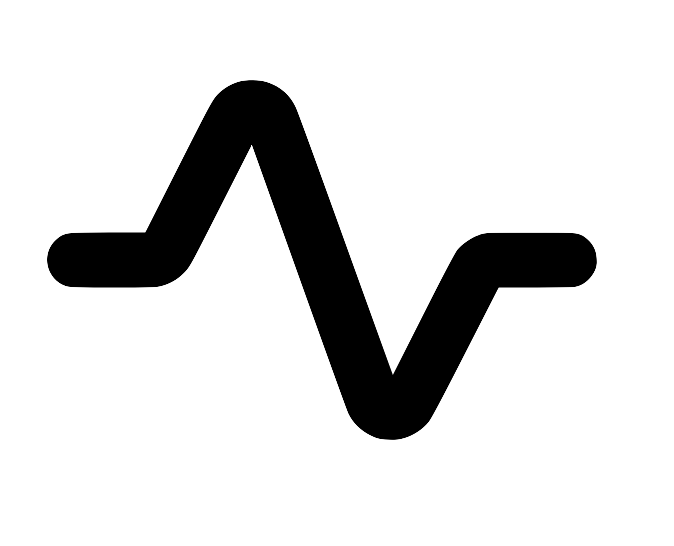
\includegraphics[width=1cm]{img/monitoring.png}};
	\draw \secondcircle node [above right, align=center,text=Purple] {
		\textbf{Architecture de }\\
		\textbf{communication}
	};
\draw node[xshift=5cm,yshift=-0.5cm,align=center] { 
	
\includegraphics[width=1.1cm]{network2.png}};

	\draw \thirdcircle node [below, align=center,text=Orange] {\textbf{Traçabilité 
	et}\\\textbf{historique des données}};

\draw node[xshift=2cm,yshift=-3.8cm,align=center] { 
	
\includegraphics[width=0.9cm]{history.png}};
	\end{scope}
	
	\node[ttt,brown,align=center] at (2,0.3)  {\textbf{Technos web}\\(intérop.)};
	\node[ttt,brown] at (0.7,-1.5)  {\textbf{\tiny Structure données}};
	
	
	\node[ttt,Purple] at (2,-0.1)  {\textbf{Robustesse}};
	\node[ttt,Purple] at (3.9,-1.8)  {\textbf{Résilience}};
	\node[ttt,Purple] at (3.4,-1.5)  {\textbf{Passage à l'échelle}};
	
	\node[ttt,Orange] at (3.4,-1.25)  {\textbf{Couplage lâche}};
	\node[ttt,Orange] at (0,-1.8)  {\textbf{Expertise}};
	\node[ttt,Purple] at (3.4,-1.5)  {\textbf{Passage à l'échelle}};
	


	\end{tikzpicture}